% !TeX program = pdflatex
% Compiler Engineering Suite - shared standalone pdfLaTeX preamble
\documentclass[10pt,letterpaper]{article}
\usepackage[T1]{fontenc}
\usepackage[utf8]{inputenc}
\usepackage{lmodern}
\usepackage[margin=.78in,headheight=18pt]{geometry}
\usepackage[table]{xcolor}
\usepackage{microtype}
\usepackage{amsmath,amssymb}
\usepackage{booktabs,longtable,array}
\usepackage{enumitem}
\usepackage{fancyhdr}
\usepackage{hyperref}
\usepackage{needspace}
\usepackage{fancyvrb}
\usepackage{tikz}
\usetikzlibrary{arrows.meta,positioning,shapes.geometric}
\definecolor{CompilerBlue}{HTML}{1F4E79}
\definecolor{CompilerInk}{HTML}{263746}
\definecolor{CompilerGray}{HTML}{52616B}
\definecolor{CompilerLight}{HTML}{EFF4F8}
\hypersetup{colorlinks=true,linkcolor=CompilerBlue,urlcolor=CompilerBlue,citecolor=CompilerBlue}
\setlength{\parindent}{0pt}
\setlength{\parskip}{6pt plus 2pt}
\setlist[itemize]{leftmargin=*,itemsep=3pt,topsep=2pt}
\setlist[enumerate]{leftmargin=*,itemsep=3pt,topsep=2pt}
\pagestyle{fancy}
\fancyhf{}
\fancyhead[L]{\small\textcolor{CompilerGray}{Compiler Engineering Documentation Suite}}
\fancyhead[R]{\small\thepage}
\renewcommand{\headrulewidth}{.4pt}
\newcommand{\evidence}[1]{\par\smallskip\noindent\textbf{Evidence required:} #1\par}
\newcommand{\sourceanchor}[1]{\textbf{Book anchor:} #1\par}
\newcommand{\modern}{\textbf{Modern engineering extension (not attributed to the source book):} }
\newcommand{\writinglines}[1]{\par\noindent\rule{\linewidth}{.3pt}\par\vspace{#1\baselineskip}\noindent\rule{\linewidth}{.3pt}\par}
\newcommand{\checkboxline}[1]{\noindent $\square$\quad #1\par}
\newcommand{\formfield}[2]{\noindent\textbf{#1}\par\vspace{#2\baselineskip}\hrule\medskip}

\hypersetup{pdftitle={Compiler Engineering Technical Handbook},pdfauthor={Compiler Engineering Documentation Suite}}
\begin{document}
\begin{titlepage}
\centering\vspace*{1.0in}
{\Huge\bfseries\textcolor{CompilerBlue}{Compiler Engineering Technical Handbook}\par}
\vspace{.22in}{\Large Pass boundaries, invariants and implementation decisions\par}
\vspace{.4in}{\large Compiler Engineering Documentation Suite\par}
\vfill
\begin{minipage}{.86\linewidth}\small
Source basis: Keith D. Cooper and Linda Torczon, \emph{Engineering a Compiler}, Third Edition (Morgan Kaufmann/Elsevier, 2023). All explanatory text, examples, questions, and implementation designs in this document are independently authored. The book is not included.\par\medskip
Document class: Technical reference.
\end{minipage}
\vfill\textcolor{CompilerGray}{Version 1.0 --- 2026-10-30}\par
\end{titlepage}
\tableofcontents\clearpage
\section{Architecture and pass contracts}
A compiler is a translation system with a front end, an intermediate representation, an optimizer and a back end (Chapter 1). Each pass must specify accepted input form, produced output form, preserved semantics, invalidated analyses and possible diagnostics.
\begin{center}
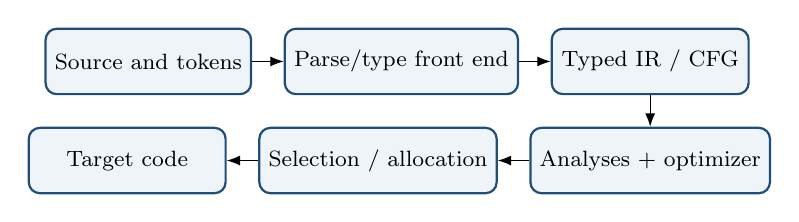
\begin{tikzpicture}[node distance=4mm and 4mm, every node/.style={font=\footnotesize}, box/.style={draw=CompilerBlue,thick,rounded corners,minimum width=2.5cm,minimum height=.83cm,fill=CompilerLight}]
\node[box] (s) {Source and tokens}; \node[box,right=of s] (f) {Parse/type front end}; \node[box,right=of f] (i) {Typed IR / CFG};
\node[box,below=of i] (o) {Analyses + optimizer}; \node[box,left=of o] (b) {Selection / allocation}; \node[box,left=of b] (t) {Target code};
\draw[-{Latex}] (s)--(f); \draw[-{Latex}] (f)--(i); \draw[-{Latex}] (i)--(o); \draw[-{Latex}] (o)--(b); \draw[-{Latex}] (b)--(t);
\end{tikzpicture}
\end{center}
\textbf{Pass contract:} preconditions, mutation footprint, invariants, analysis invalidations, failure path, deterministic tests.

\section{Language semantics as an optimization boundary}
\begin{itemize}
\item Preserve observable behavior, including side effects and exception ordering.
\item Do not assume integer overflow is algebraically interchangeable across source languages.
\item Floating-point reassociation can change rounding and exceptional values.
\item Declare the memory model and alias assumptions before code motion.
\item Maintain diagnostic span provenance during front-end lowering.
\end{itemize}

\section{Data structure invariants}
\begin{longtable}{|p{0.18\linewidth}|p{0.44\linewidth}|p{0.31\linewidth}|}
\hline
Artifact & Correctness invariant & Mutation check\\ \hline\endfirsthead
\hline
Artifact & Correctness invariant & Mutation check\\ \hline\endhead
Tokens & Monotone source span with explicit EOF & Reject overlapping source spans\\ \hline
AST & Every node has a defined operator and child arity & Validate recursively\\ \hline
CFG & Edges agree with block terminators & Recompute successors and predecessors\\ \hline
SSA & Every use is dominated by its definition (phi uses on incoming edges) & Verify dominance and phi predecessor count\\ \hline
Interference graph & Edges encode simultaneous liveness & Recompute after rewriting live ranges\\ \hline
\end{longtable}

\section{Algorithm-to-evidence decision table}
\begin{longtable}{|p{0.23\linewidth}|p{0.46\linewidth}|p{0.24\linewidth}|}
\hline
Pass/technique & Correctness witness & Cost driver\\ \hline\endfirsthead
\hline
Pass/technique & Correctness witness & Cost driver\\ \hline\endhead
NFA to DFA & Acceptance equivalence on representative alphabet classes & Subset-state explosion\\ \hline
LL(1) parser & FIRST/FOLLOW and conflict-free parse table & Grammar/table size\\ \hline
Iterative liveness & Transfer equations at a fixed point & CFG edges x iterations\\ \hline
Tree-pattern selection & Legal cover and target-cost objective & Pattern count, tree size\\ \hline
List scheduler & Topological order with resource/latency constraints & Ready-queue size\\ \hline
Graph-color allocator & No interfering virtual registers share a physical register & Edges, spills, recoloring\\ \hline
\end{longtable}

\section{Traceability to source}
The book\textquotesingle s Chapter 1 introduces the compiler pipeline; Chapters 2--3 describe scanner/parser construction; Chapters 4--7 connect source programs to IR; Chapters 8--10 address optimization; Chapters 11--13 address back-end algorithms; Chapter 14 addresses runtime optimization. Appendices A and B cover ILOC and supporting data structures.

\end{document}
